\chapter{Case Study}
\thispagestyle{plain}

\section{Instance description}
In this chapter, we present a case study of a well known scheduling instance from \cite{KONDILI1993211}, optimized for the deterministic case using the described online tool. The production of two products 1 and 2 from three feed stocks A, B and C takes place according to the STN representation given in Fig. \ref{fig:STN}. This instance has four intermediate states and five tasks.

\begin{figure}[htbp]
\centering
\fbox{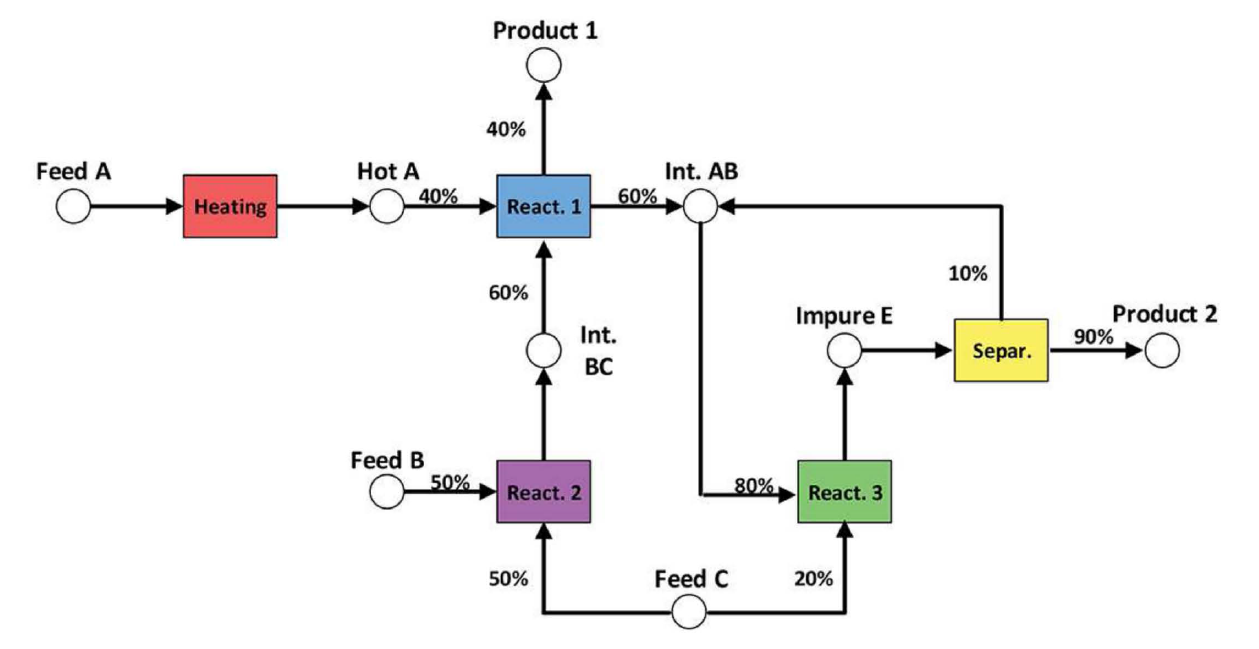
\includegraphics[width=\linewidth]{Images/STN.png}}
\caption{State task network for the example instance}
\label{fig:STN}
\end{figure}

Table \ref{tab:statelevels} shows the state maximum capacity and initial load data for the problem. The available unit, task compatibility and processing time data is given in Table \ref{tab:tasks}.

\begin{table}[htb]
\centering
\caption{Problem data (states)}
\label{tab:statelevels}
\begin{tabular}{@{}cccc@{}}
\toprule
\textbf{State} & \textbf{Capacity} & \textbf{Initial load} & \textbf{Price (per unit)} \\ \midrule
Feed A         & 1000              & 1000                  & -                         \\
Feed B         & 1000              & 1000                  & -                         \\
Feed C         & 1000              & 1000                  & -                         \\
Hot A          & 100               & -                     & -                         \\
Int. BC        & 200               & -                     & -                         \\
Int. AB        & 150               & -                     & -                         \\
Impure E       & 200               & -                     & -                         \\
Product 1      & 1000              & -                     & 10                        \\
Product 2      & 1000              & -                     & 10                        \\ \bottomrule
\end{tabular}
\end{table}

\begin{table}[htb]
\centering
\caption{Problem data (units \& tasks)}
\label{tab:tasks}
\begin{tabular}{@{}ccccccccc@{}}
\toprule
Unit         & \multicolumn{2}{c}{Heater} & \multicolumn{2}{c}{Reactor 1} & \multicolumn{2}{c}{Reactor 2} & \multicolumn{2}{c}{Separator} \\ \cmidrule(l){2-9} 
Maximum Load & \multicolumn{2}{c}{100}    & \multicolumn{2}{c}{50}        & \multicolumn{2}{c}{80}        & \multicolumn{2}{c}{200}       \\ \midrule
Tasks        & $\alpha$       & $\beta$       & $\alpha$         & $\beta$        & $\alpha$         & $\beta$        & $\alpha$         & $\beta$        \\ \cmidrule(l){2-9} 
Heating      & 0.667        & 0.007       &                &              &                &              &                &              \\
Reaction 1   &              &             & 1.334          & 0.027        & 1.334          & 0.017        &                &              \\
Reaction 2   &              &             & 1.334          & 0.027        & 1.334          & 0.017        &                &              \\
Reaction 3   &              &             & 0.667          & 0.013        & 0.667          & 0.008        &                &              \\
Separation   &              &             &                &              &                &              & 1.334          & 0.007        \\ \bottomrule
\end{tabular}
\end{table}

\section{Defining instance parameters}
\subsection{Defining units}
\begin{figure}[htb]
\centering
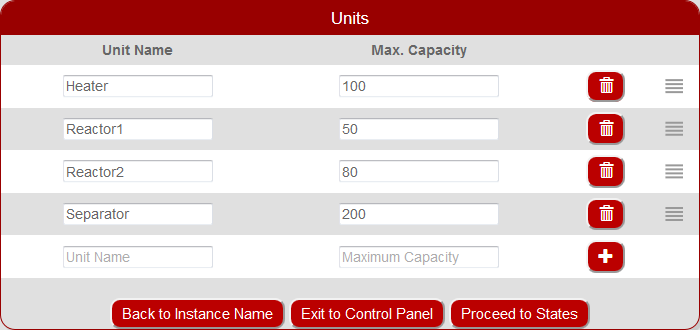
\includegraphics[width=\linewidth]{Images/DefineUnits.png}
\caption{Units input into webtool}
\label{fig:defUnits}
\end{figure}
Unit names and maximum capacities from Table \ref{tab:tasks} are input into the units table of the web tool as shown in Fig. \ref{fig:defUnits}.



\subsection{Defining states}
\begin{figure}[htbp]
\centering
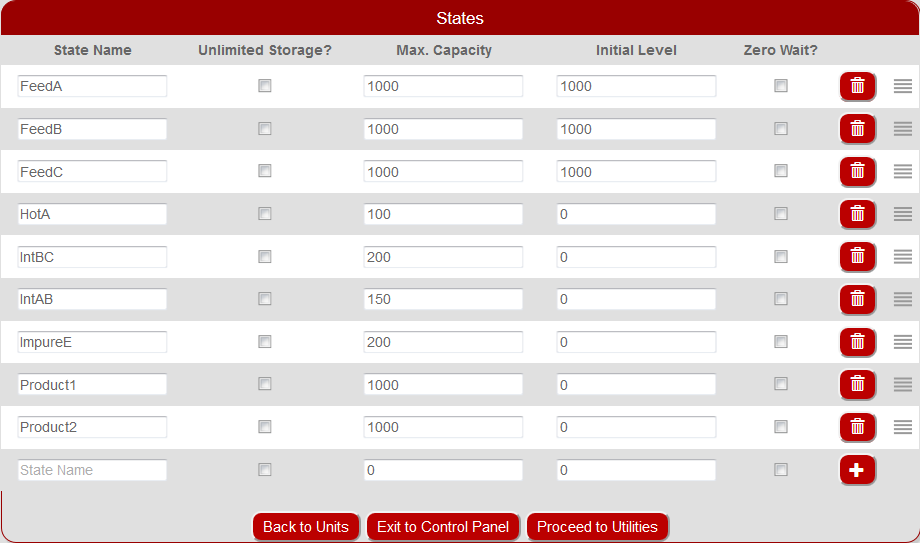
\includegraphics[width=\linewidth]{Images/DefineStates.png}
\caption{States input into webtool}
\label{fig:defStates}
\end{figure}
State names, maximum storage capacities and initial levels from Table \ref{tab:statelevels} are input into the units table of the web tool as shown in Fig. \ref{fig:defStates}.


\subsection{Defining tasks}
\begin{figure}[htb]
\centering
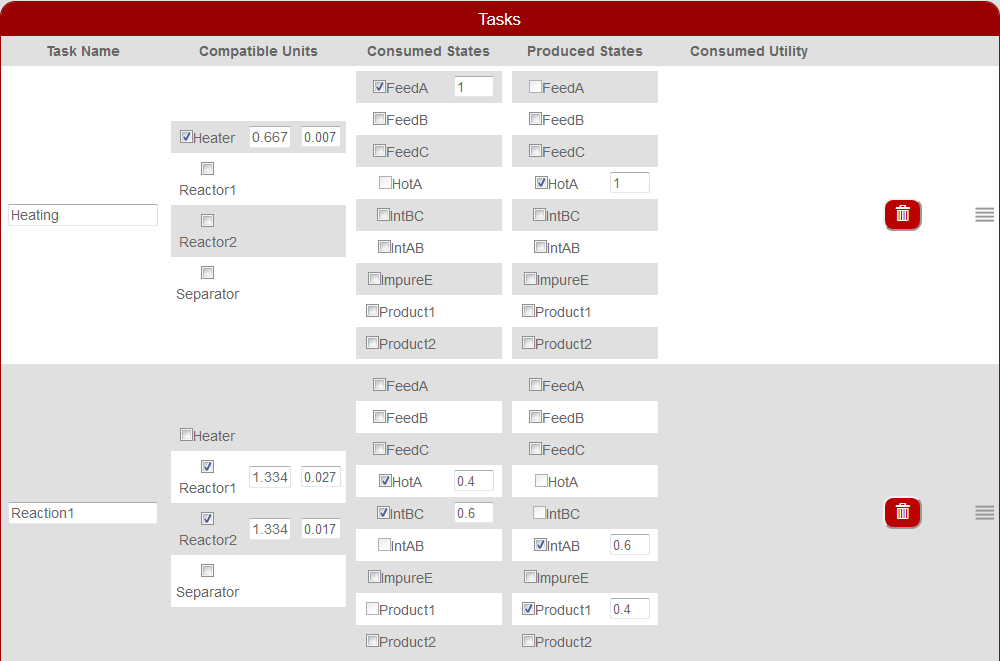
\includegraphics[width=\linewidth]{Images/DefineTasks.png}
\caption{Tasks input into webtool}
\label{fig:defTasks}
\end{figure}

This instance does not involve utilities. Hence we can skip utilities input. For each task in Table \ref{tab:tasks}, the values of $\alpha$ and $\beta$ are input after selecting the appropriate compatible unit(s). Fig. \ref{fig:defTasks} shows the tasks table after successful input of tasks Heating and Reaction 1.


\subsection{Objective}

\begin{figure}[htb]
\centering
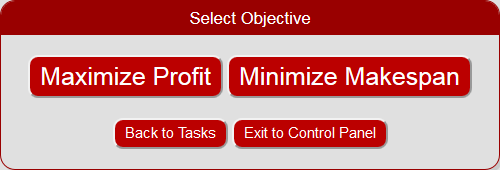
\includegraphics[width=0.8\linewidth]{Images/DefineObjective.png}
\caption{Objective selection}
\label{fig:selectObjective}
\end{figure}

For this case, we will consider the case of maximization of profit. After successful completion of the tasks input, the objective selection options are available as shown in Fig. \ref{fig:selectObjective}. After clicking on ``Maximize profit'', the horizon and price input screen appears as shown in Fig. \ref{fig:prices}. The instance definition is complete after input of horizon and price data for Product 1 and Product 2 from Table \ref{tab:statelevels}. We will consider an 8 hour horizon for this case study.

\begin{figure}[htb]
\centering
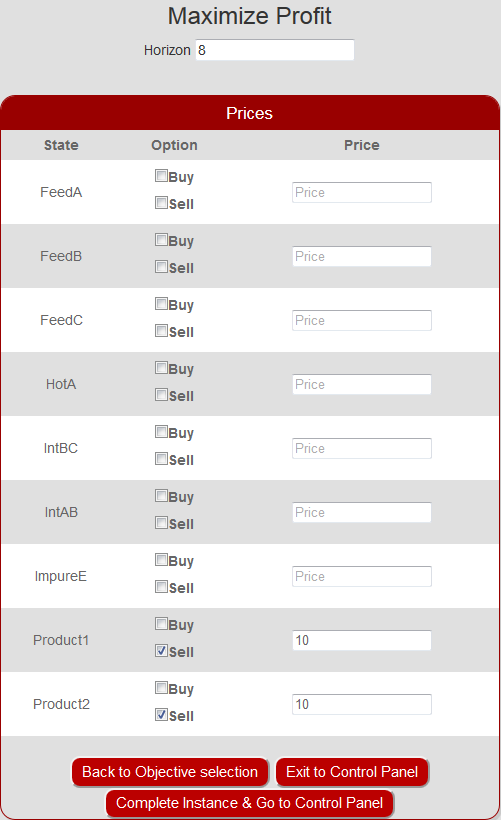
\includegraphics[width=0.8\linewidth]{Images/Prices.png}
\caption{Horizon and price input}
\label{fig:prices}
\end{figure}

\subsection{Model and event points}





